\documentclass{article}
\usepackage[utf8]{inputenc}
\usepackage{graphicx}
\graphicspath{ {./images/} }

\author{Mikołaj Walczak}
\title{Semantic relations in embeddings}

\begin{document}
  \maketitle
  \section{T-SNE visualization}
  \begin{figure}[ht]
    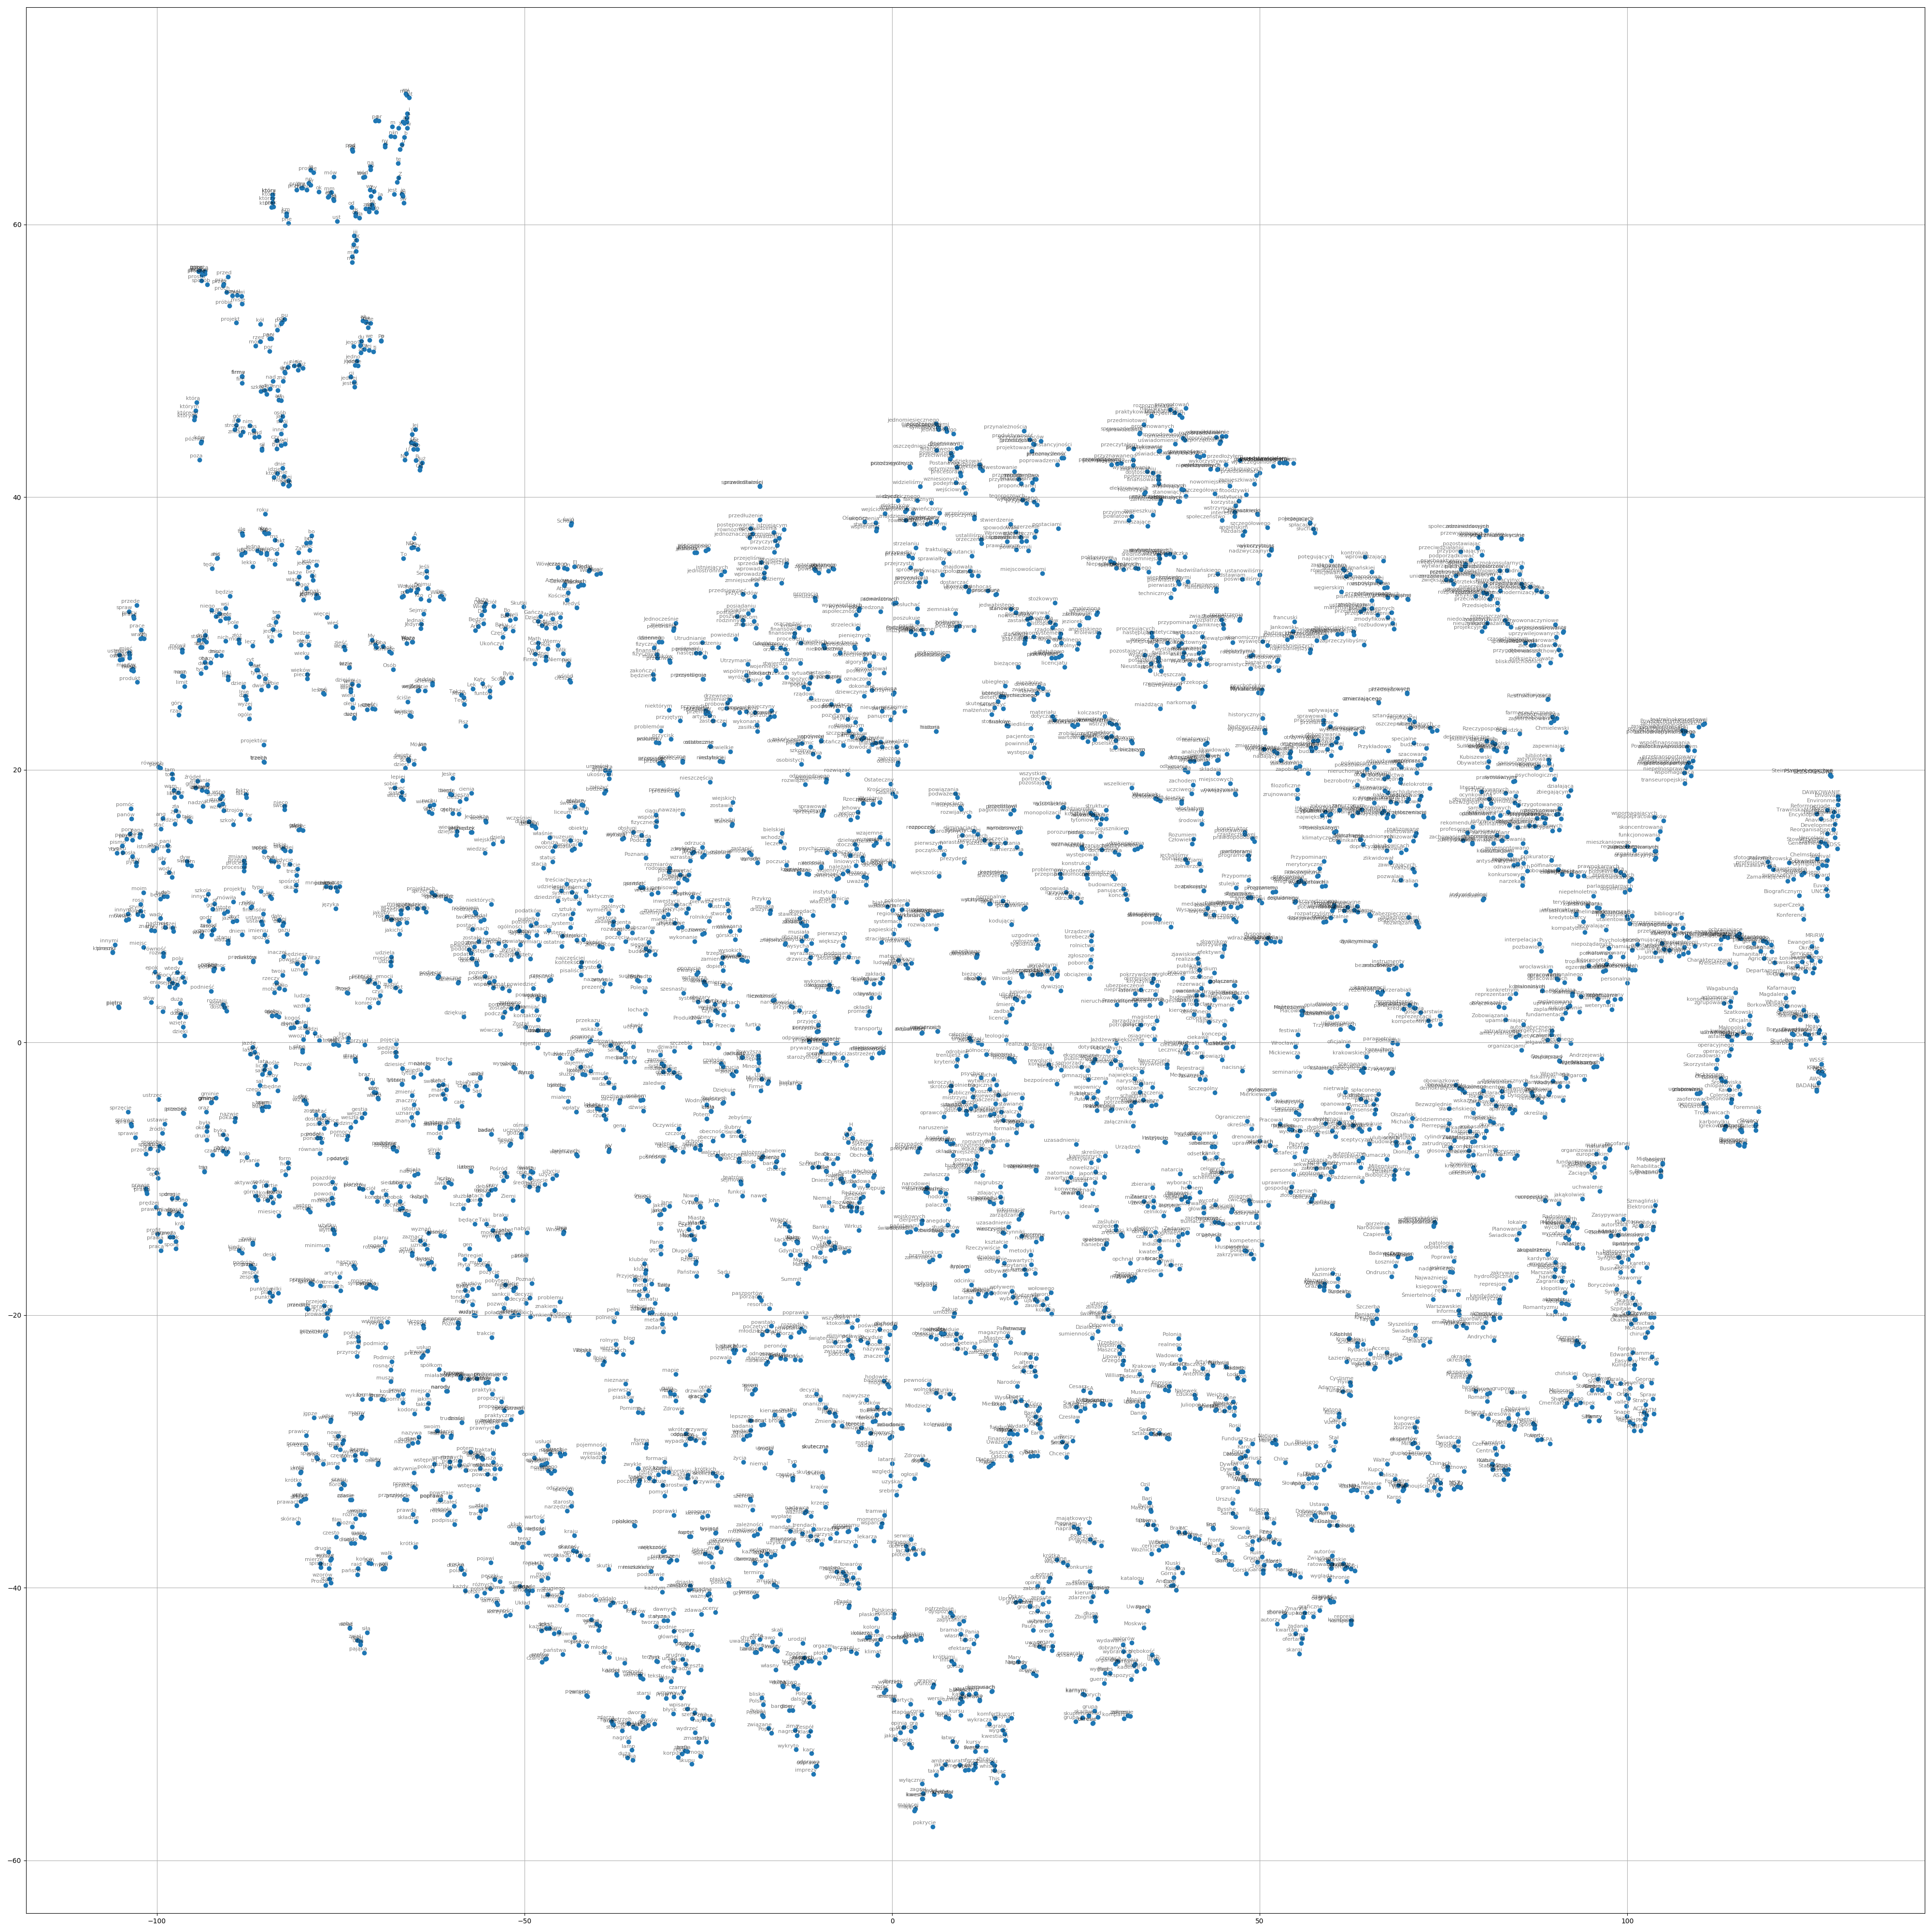
\includegraphics[width=\textwidth]{embeddings_500}
    \caption{T-SNE visualization of the first 500 words from the corpus}
    \label{fig:tsne-500}
  \end{figure}

  \section{Singular-Plural relation}
  By analizing the t-sne visualizations the most noticable relation at the first
  glance was how closely singular and plural forms of the same noun occurred on
  the graph. I have decided to analyze if we can extract a vector $\delta$ such that
  for any nouns $s$ and $p$ such that $p$ is a plural form of a noun $s$ the
  following equation holds:
  \begin{equation}
    s + \delta \approx p
  \end{equation}

  \subsection{Definitions}
  For convinience lets define a relation of being a plural
  \begin{equation}
    P = \{\langle s, p \rangle : \textrm{$p$ is a plural of $s$} \}
  \end{equation}
  Next for each pair $\langle s, p \rangle \in P$  we define a difference vector
  \begin{equation}
    \delta_{\langle s, p \rangle} = p - s
  \end{equation}

  \subsection{Results}
  A set of words has been extracted to check if the relation holds. For each
  $\langle s, p \rangle \in P$ and $\langle s', p' \rangle \in P$ the cosine
  similarity has been calculated between $s' + \delta_{\langle s, p \rangle}$
  and $p'$. Partial results can be seen in the table below (\ref{tab:sinpl_sim}),
  where for readability words has been replaced with $s_i$ and $p_i$ as explained
  in the table \ref{tab:sinpl_set}

  \begin{table}[ht]
    \center
  \begin{tabular}{|l|c|c|c|c|c|}
  \hline
    $\delta$ & $s_1 + \delta \approx p_1$ & $s_2 + \delta \approx p_2$ & $s_3 + \delta \approx p_3$  & $s_4 + \delta \approx p_4$  & $s_5 + \delta \approx p_5$ \\ \hline
    $\delta_{\langle s_1, p_1 \rangle}$ & 1.0000 & 0.9832 & 0.9995 & 0.9969 & 0.9993 \\ \hline
    $\delta_{\langle s_2, p_2 \rangle}$ & 0.9807 & 1.0000 & 0.9933 & 0.9788 & 0.9983 \\ \hline
    $\delta_{\langle s_3, p_3 \rangle}$ & 0.9977 & 0.9762 & 1.0000 & 0.9925 & 0.9991 \\ \hline
    $\delta_{\langle s_4, p_4 \rangle}$ & 0.9978 & 0.9840 & 0.9988 & 1.0000 & 0.9990 \\ \hline
    $\delta_{\langle s_5, p_5 \rangle}$ & 0.9944 & 0.9890 & 0.9985 & 0.9878 & 1.0000 \\ \hline
  \end{tabular}
  \caption{Cosine similarity between singular and plural forms}
  \label{tab:sinpl_sim}
  \end{table}

  \begin{table}[ht]

      \center
  \begin{tabular}{|l|c|c|}
  \hline
  $i$ & $s_i$ & $p_i$ \\ \hline
  1 & strata & straty \\ \hline
  2 & miejsce & miejsca \\ \hline
  3 & umowa & umowy \\ \hline
  4 & firma & firmy \\ \hline
  5 & odprawa & odprawy \\ \hline
  \end{tabular}
  \caption{Set of singular and plural forms}
  \label{tab:sinpl_set}
  \end{table}

\end{document}
